\documentclass[12pt]{article}

\title{3XA3 Development Plan Group 3}
\author{Yousaf Shaheen, Jason Li, Scott Williams}
\date{Sept 28, 2017}
\usepackage{graphicx}
\usepackage{indentfirst}
\graphicspath{{img/}}


\begin{document}

\vspace*{7\baselineskip}
\begin{center}
\begin{large}
\textbf{Group 3 Development Plan} \\
\end{large}
Project: Hextris \\
Team Members: Yousaf Shaheen, Jason Li, Scott Williams \\
Professor: Asghar Bokhari \\
Date: Sept 28, 2017 \\
Course: 3XA4  \\
\end{center}

\newpage
\tableofcontents
\newpage



\section{Introduction and Project Team}
This document outlines the Development plan of the Project. It contains details of how the project will be completed. It outlines the process in which the documentation will be produced and contains implementation details. This document also includes scheduling aspects of the project.


\subsection{Team Member Roles}
Members will be given prominent roles in which they are comfortable in but are not restricted to fulfilling the requirement alone.\\

\textbf{Yousaf Shaheen - Latex, Doxygen}\\
	- creation of Latex files and pdfs for all documents and submissions\\
 	- majority of documentation and document generation\\
 	
\textbf{Scott Williams - Git, Scribe, Testing}\\
	-git processes, tags, branches and general organization\\
	-logs of meetings and recording \\
	-unity testing and C\# script testing\\
       
\textbf{Jason Li - Unity, Team Leader} \\
	- script and visual implementation in unity\\
	- coordination of group members and ensuring all aspects are completed \\


\subsection{Team Meeting Plan}
The team will meet regularly during the regular Monday and Tuesday labs. Additionally we will have separate meeting Wednesdays for 2 hours anywhere between 2:30 and 7:00 at Thode Library or a private meeting room at the Hatch Center. There will also be fill in meetings for when extra work needs to be done. These will be arranged via messenger contact between the members.

\newpage

\subsection{Team Communication Plan}
The main source of communication between team members is Facebook messenger. Facebook messenger chat group is a simple and easy way of communication for normal discussion, which also allows basic sharing of links and information. Additionally backup communication takes place in the form of text or calls, is for a more direct means for when immediate communication is needed. Phone numbers have already been shared between group members. Sharing and reviewing programming work will be through Gitlab, as it has the appropriate tools to be time efficient while working in parallel with each other. The operations that Git provides include the production of different branches and adjusting the master through re-basing. 


\section{Project Overview}
This project will recreate the game Hextris with some new additions to the game. The main purpose of this project is to gain knowledge and experience in developing a project and producing the correct documentation needed for said project. This project will give the team members a better understanding of the process of creating a program such as a game.

\subsection{Proof of Concept}
Risks and implementation:\\

The most difficult part of implementation will be the organization and manipulation of blocks falling as part of the game. Arranging them to fall towards a center point assuming a specific shape to fill a hexagon or octagon will be the most difficult part to implement. The implementation will be done on Unity which has an engine that supports many aspects of the game already including physics, 2D bodies, control manipulation. The main challenge will be to use these provided tools and manipulate them to recreate an improved version of Hextris.io. Additionally another challenge will be the extra features/modes added to the existing version. This involves additional use of the different shape libraries for 2D bodies within the unity engine.

The proof of concept as a result of the difficulty of creation of hexagons will focus on the rotation of a center hexagon, as well as a menu system that allows the application to quit, return to the start screen, and start a game session. The game session will not focus on the point system in the Proof of Concept due to the fact that block generation is not set. 

\subsection{Git Workflow Plan}
The gitflow surrounding this project will revolve around making modifications to a centralized repository that contains the master and develop branches that are in parallel with each other.\\

We will follow the workflow of creating feature branches, release branches, and hotfix branches in order to organize a series of builds for the Hextris project leading up to different milestones. The milestones in question include the Proof of Concept demonstration with the TA and professor stakeholders, as well as the final project demonstration with the end-user stakeholders that were outlined in our Problem Statement. \\

For these supporting branches, the feature branches will serve as marking points relating to key aspects of the Hextris recreation leading up to the Proof of Concept demonstration in the week of October 16th. The feature branches will consist of different versions of the project, such as one consisting of simply the hexagonal object being able to be manipulated through presses of the arrow keys on the keyboard. Another one will feature the falling blocks, with a further feature branch consisting of a Unity project being able to detect a match of three similar colored blocks being connected to each other. In this sense, the workflow model will be able to support incremented steps that can be merged back to the develop branch and further into the master branch when these features are able to be considered as a release branch. \\

After the Proof of Concept demonstration, the feature branches will mainly be used to incorporate new additions in order to fulfill the problem that was posed by the professor. In this case, each successive release branch will consist of new functionality within the context of the game. An example of this would be one dedicated to the introduction of power ups based on score of the user.\\

Hotfix branches will be created in the event of the master branch project files including significant bugs that need to be addressed before the major deliverable deadlines. This will be the case before and after the Proof of Concept leading up to the final demonstration at the end of the semester. \\

\newpage

\subsection{Testing}
Test will not present a challenge as Hextris is a fairly straightforward game in its base. Specific sections of the game must however be individually tested. These include the score counter, block generation, block elimination, powerups, and player controls.\\

Extra Considerations: All additional assets for our project will exist in the form of assets in a unity package. They will be easily accessible to anyone with a computer that is able to download the free unity engine 

\subsection{Coding Style}
The commenting that will be done inside the C\# project files will be a combination between standard, simplistic notes for specific lines of code and Doxygen-style commenting to produce well organized documentation.\\

Each line length will not exceed above characters such that they cannot fit within a standard Window on a laptop screen. This is to make it so that we don’t have to scroll sideways to check what certain processes are trying to accomplish. Additionally, the code must be legible in a way that whitespace and tab characters are used so that nested processes are tabbed to the right. For example, in a nested for loop, the innermost for loop must be indented, along with everything inside it to maintain the tabular structure we are going for. \\

Preferably, the curly braces should be cuddled around else statements similar to Mozilla’s coding structure in order to establish a clear standard for creating conditional statements in our code. \\

	CamelCase variable naming is mandatory from all team members when naming the different variables necessary to complete the program. This is not too much of a worry, as it is second nature for everyone involved. \\
	
	Finally, when using commas and parentheses, it will be important to make sure there is a little bit of whitespace between them to make sure everything is not condensed to the point that it makes reviewing code a hassle for the group. 


\subsection{Technology}
The project will be build on the unity game engine platform, this gives us easy access to many prebuilt functionalities such as physics engines and drawing. Additionally it gives us the option to create our own visuals when we add additional content to the game. The language used will be C\# as it is the most familiar language to the group members amongst the 2 supported for unity. Scripts for the game will be written in Visual Studio for the most part with group member Scott writing scripts in MonoDevelop. Unity, Visual Studio, and MonoDevelop all have their own testing framework (Unity test tools, Microsoft Unit Test, NUnit) that will allow us to test everything from our C\# scripts to our game features. For document generation since we are using C\# we will be using Doxygen for document generation. The tools selected for testing and document generation have been chosen for ease of use and compatibility as they were made for the platforms we are using. 


\section{Scheduling (Gantt Chart)}
The following is a Gantt Project chart detailing the project schedule.
\begin{figure}[h!]
\centering
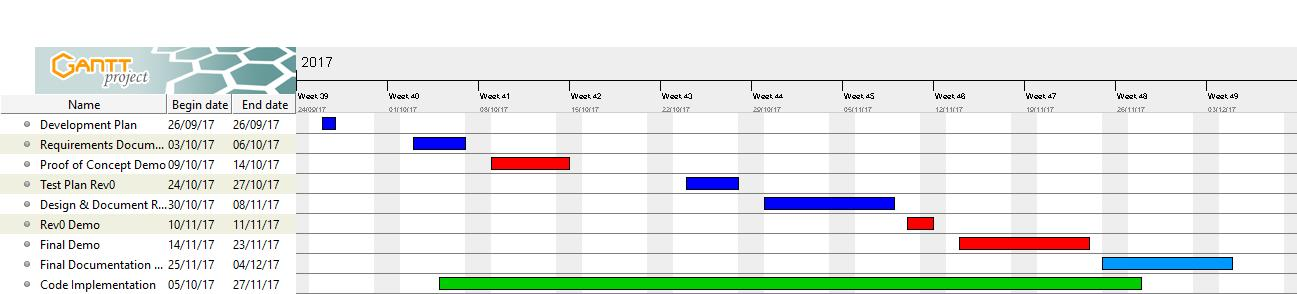
\includegraphics[width = 14cm, height = 6cm]{GanttChart}
\caption{Gantt Chart}
\end{figure}


\end{document}